\section{Architecture}

\subsection{Assessing Contribution Quality}

\begin{frame}{Existing Solutions}

  \begin{columns}[T]
    
    \begin{column}{.33\textwidth}
      \small\centering
      \textbf{Server-side evaluation}~\autocite{zhou_DifferentiallyPrivateFederated_2022}

      \begin{figure}
        \centering
        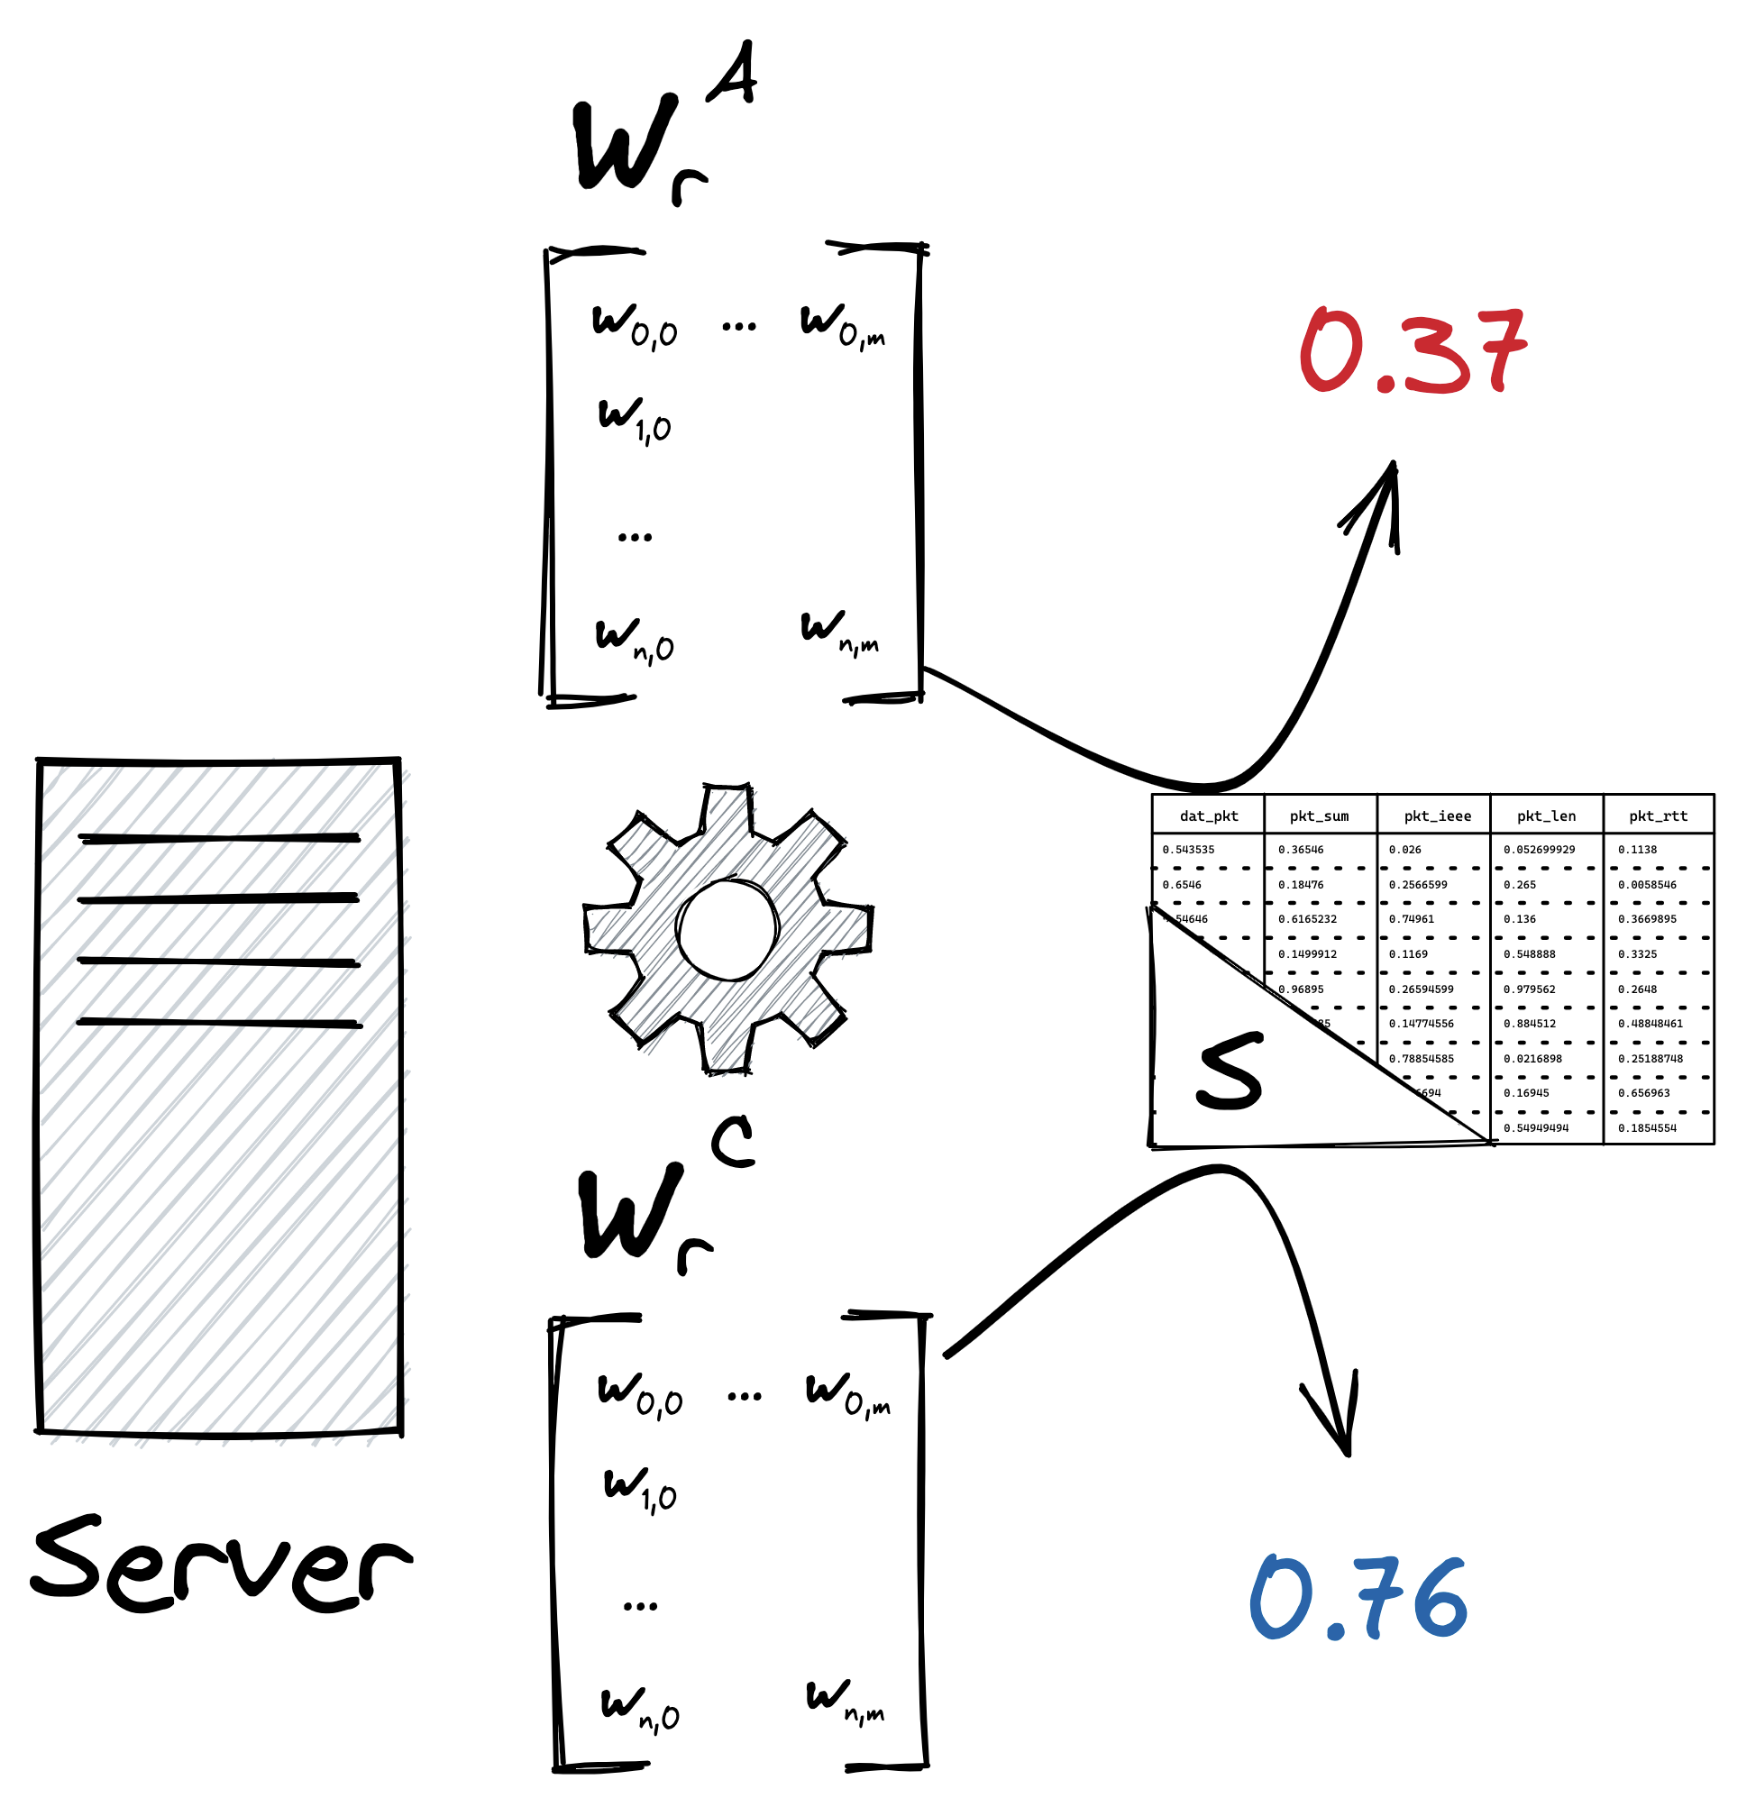
\includegraphics[height=.36\textheight]{figures/radar/server-side-eval}
      \end{figure}

      \begin{itemize}\smaller
        \item Only applicable in IID settings.
        \item Single source of truth.
      \end{itemize}
    \end{column}

    \onslide<2->{%
      \begin{column}{.33\textwidth}
        \small\centering
        \textbf{Server-side comparison}~\autocite{briggs_Federatedlearninghierarchical_2020}

        \begin{figure}
          \centering
          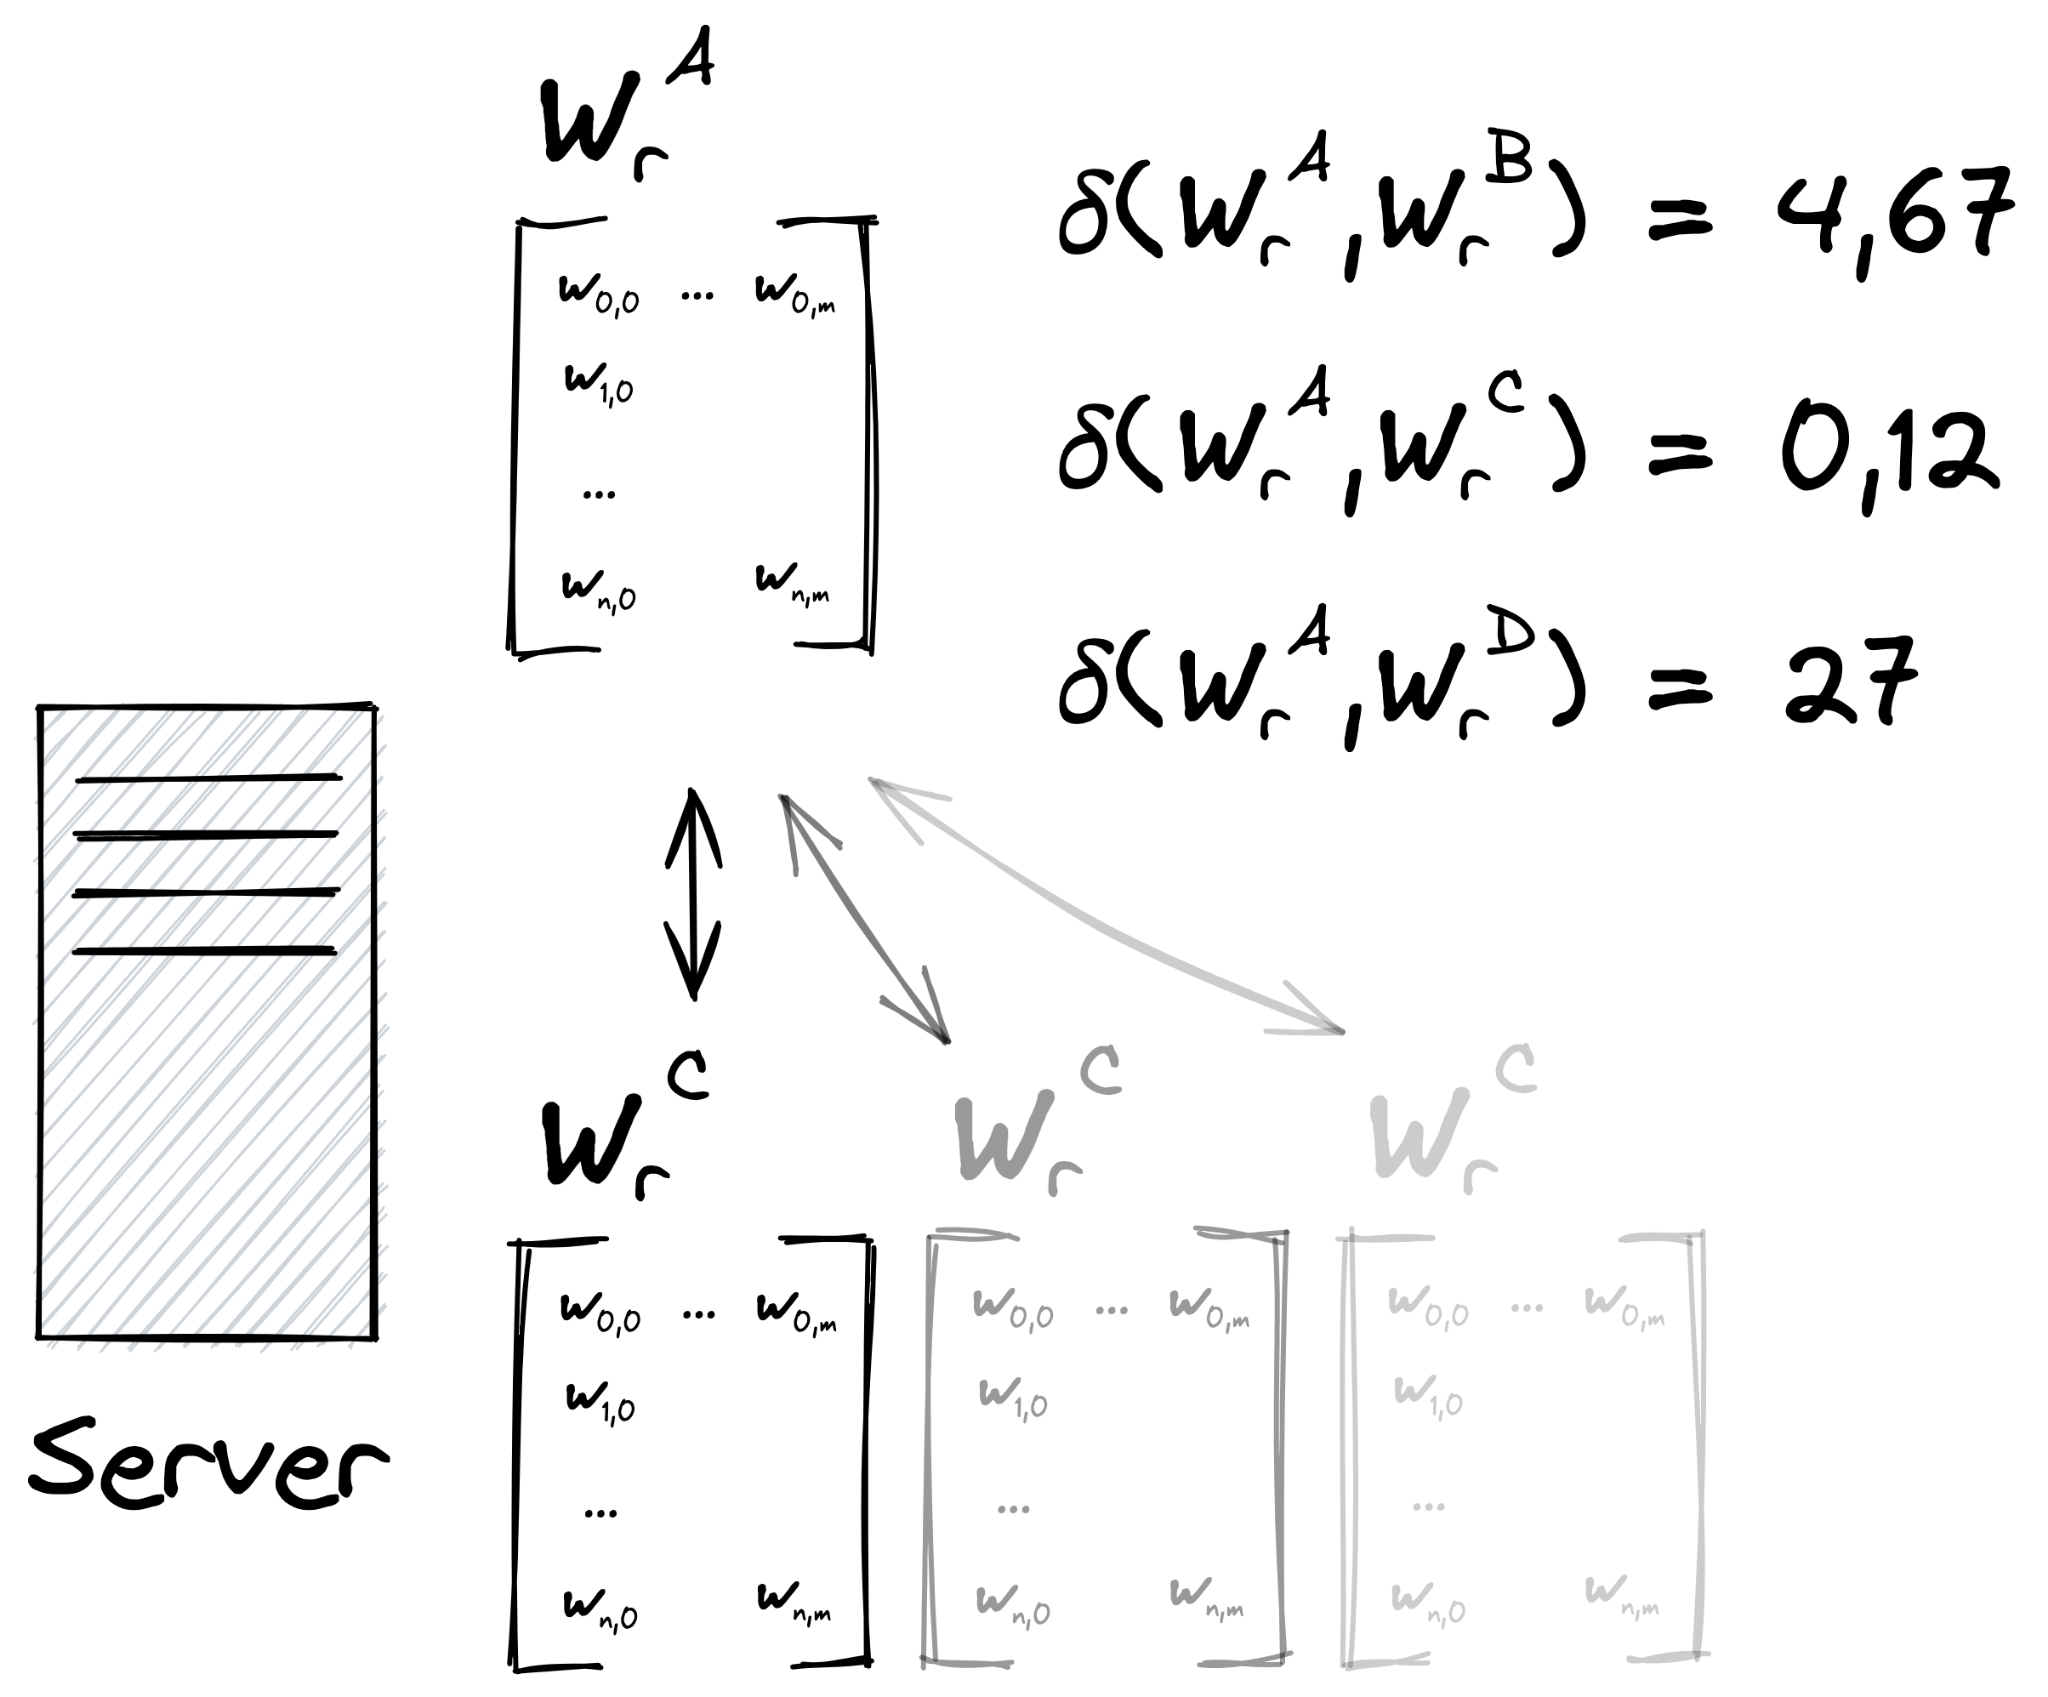
\includegraphics[height=.36\textheight]{figures/radar/server-side-comp}
        \end{figure}

        \begin{itemize}\smaller
          \item Less related to client data.
          \item More appropriate for high-dimensional data.
        \end{itemize}
      \end{column}%
    }

    \onslide<3->{%
      \begin{column}{.33\textwidth}
        \small\centering
        \textbf{Client-side evaluation}~\autocite{zhao_ShieldingCollaborativeLearning_2020}

        \begin{figure}
          \centering
          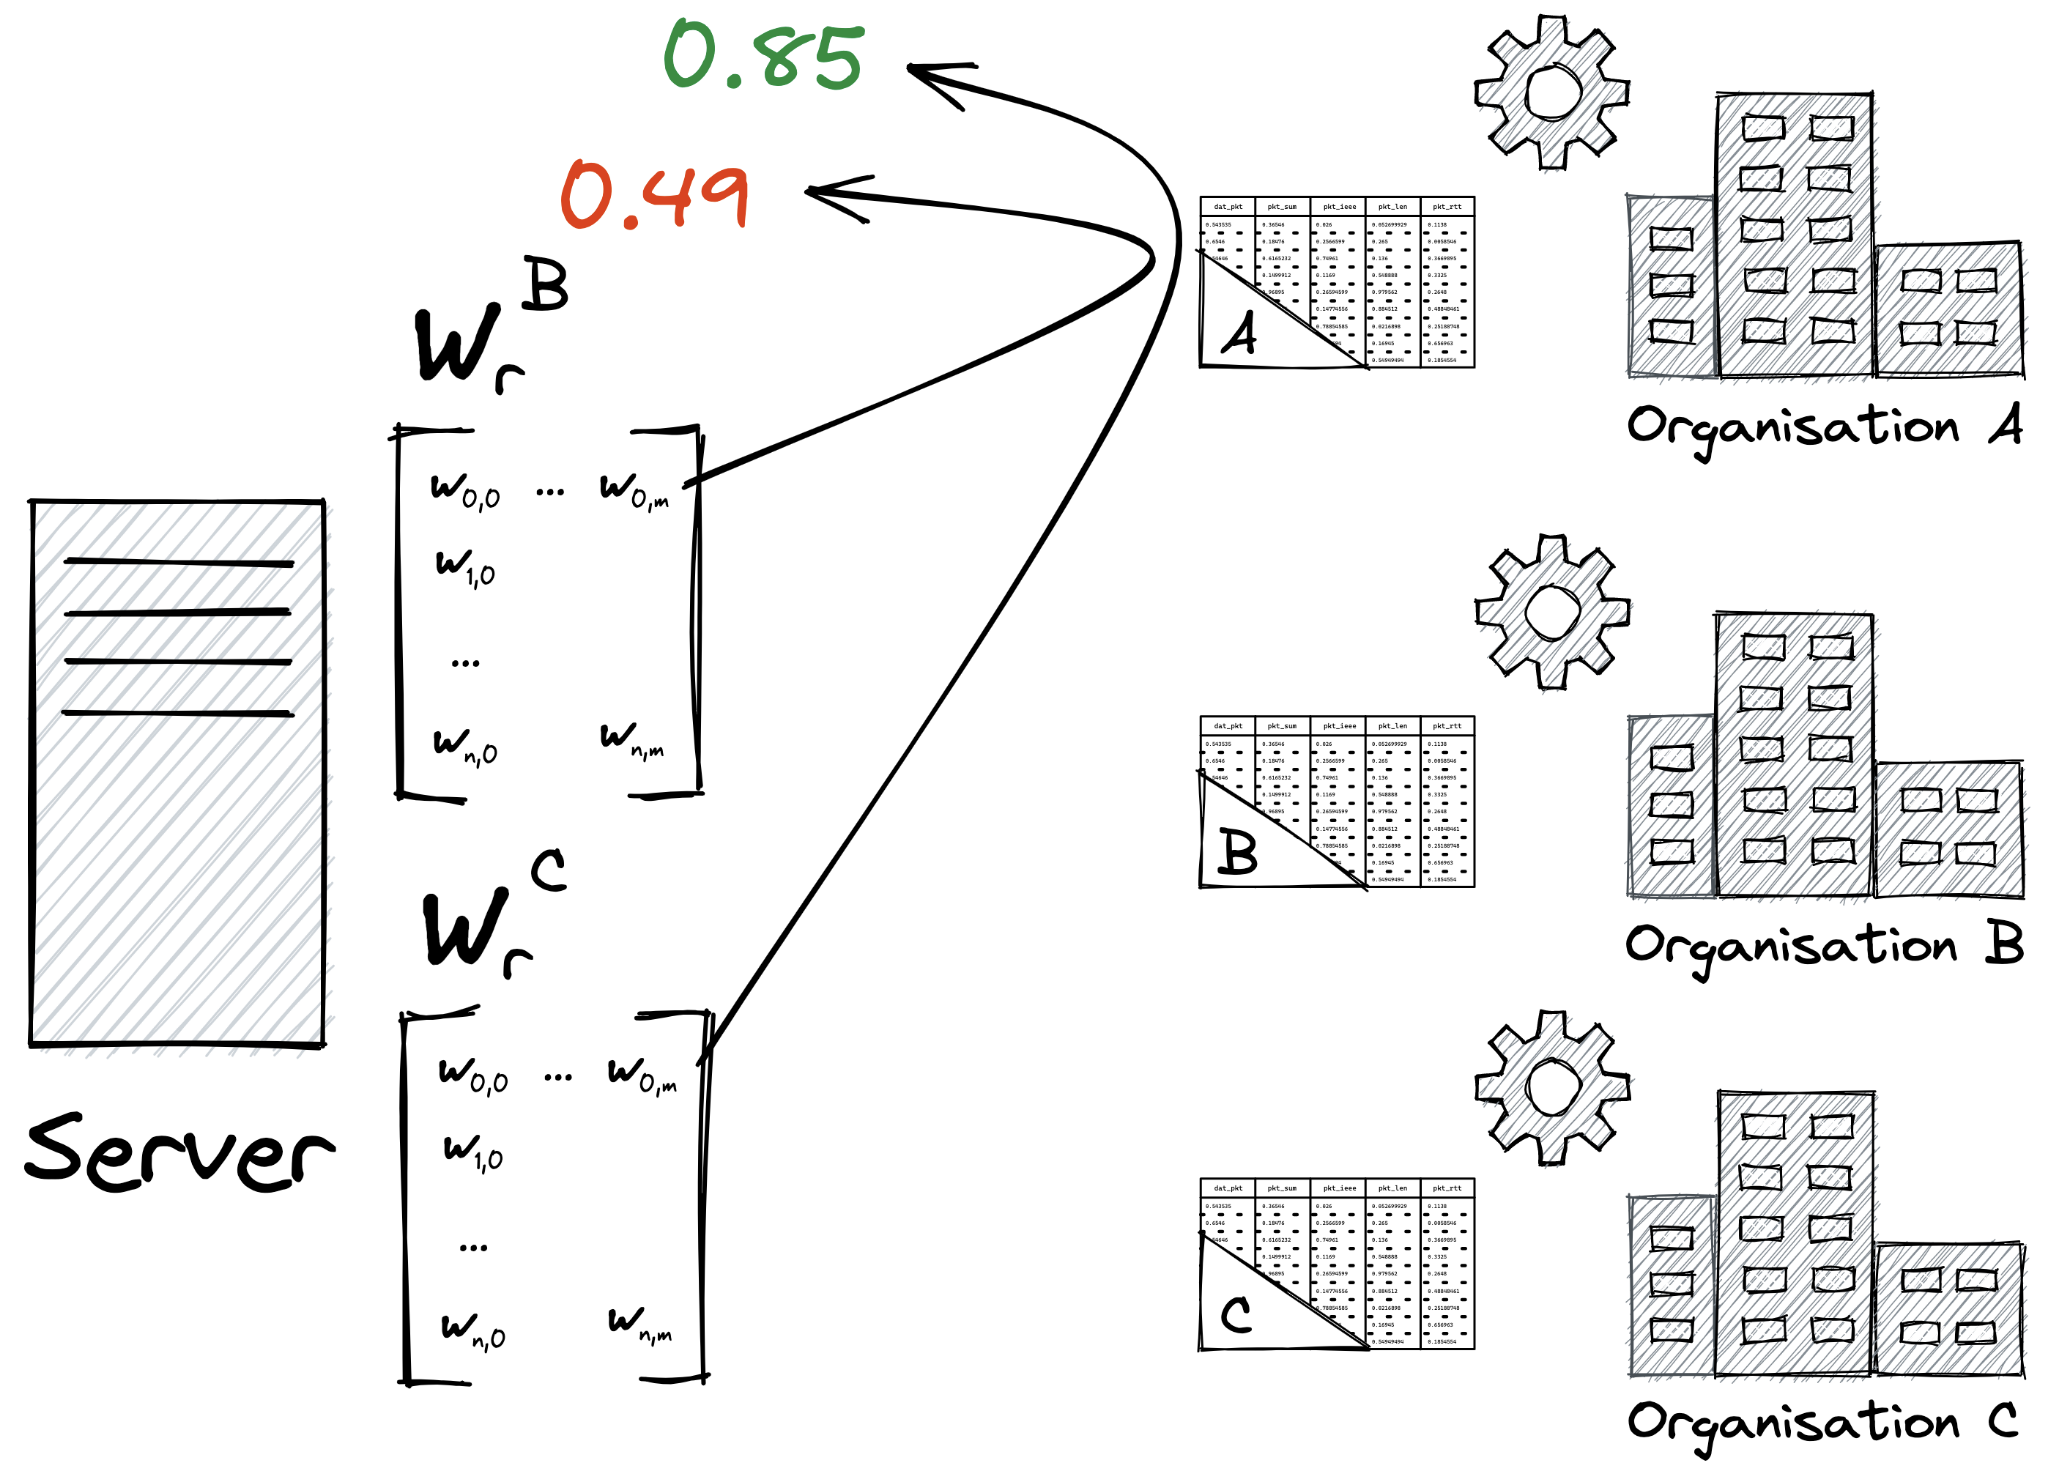
\includegraphics[height=.36\textheight]{figures/radar/client-side-eval}
        \end{figure}

        \begin{itemize}\smaller
          \item High cost in cross-device.
          \item More susceptible to badmouthing.
        \end{itemize}
      \end{column}%
    }

  \end{columns}

  \vspace{3ex}
  
  \fcitefootnote{zhou_DifferentiallyPrivateFederated_2022}
  \only<2->{\fcitefootnote{briggs_Federatedlearninghierarchical_2020}}
  \only<3->{\fcitefootnote{zhao_ShieldingCollaborativeLearning_2020}}

\end{frame}

\begin{frame}{Assessing Quality with Cross-Evaluation}

  \begin{columns}
    \begin{column}{.45\textwidth}
      \begin{figure}
        \centering
        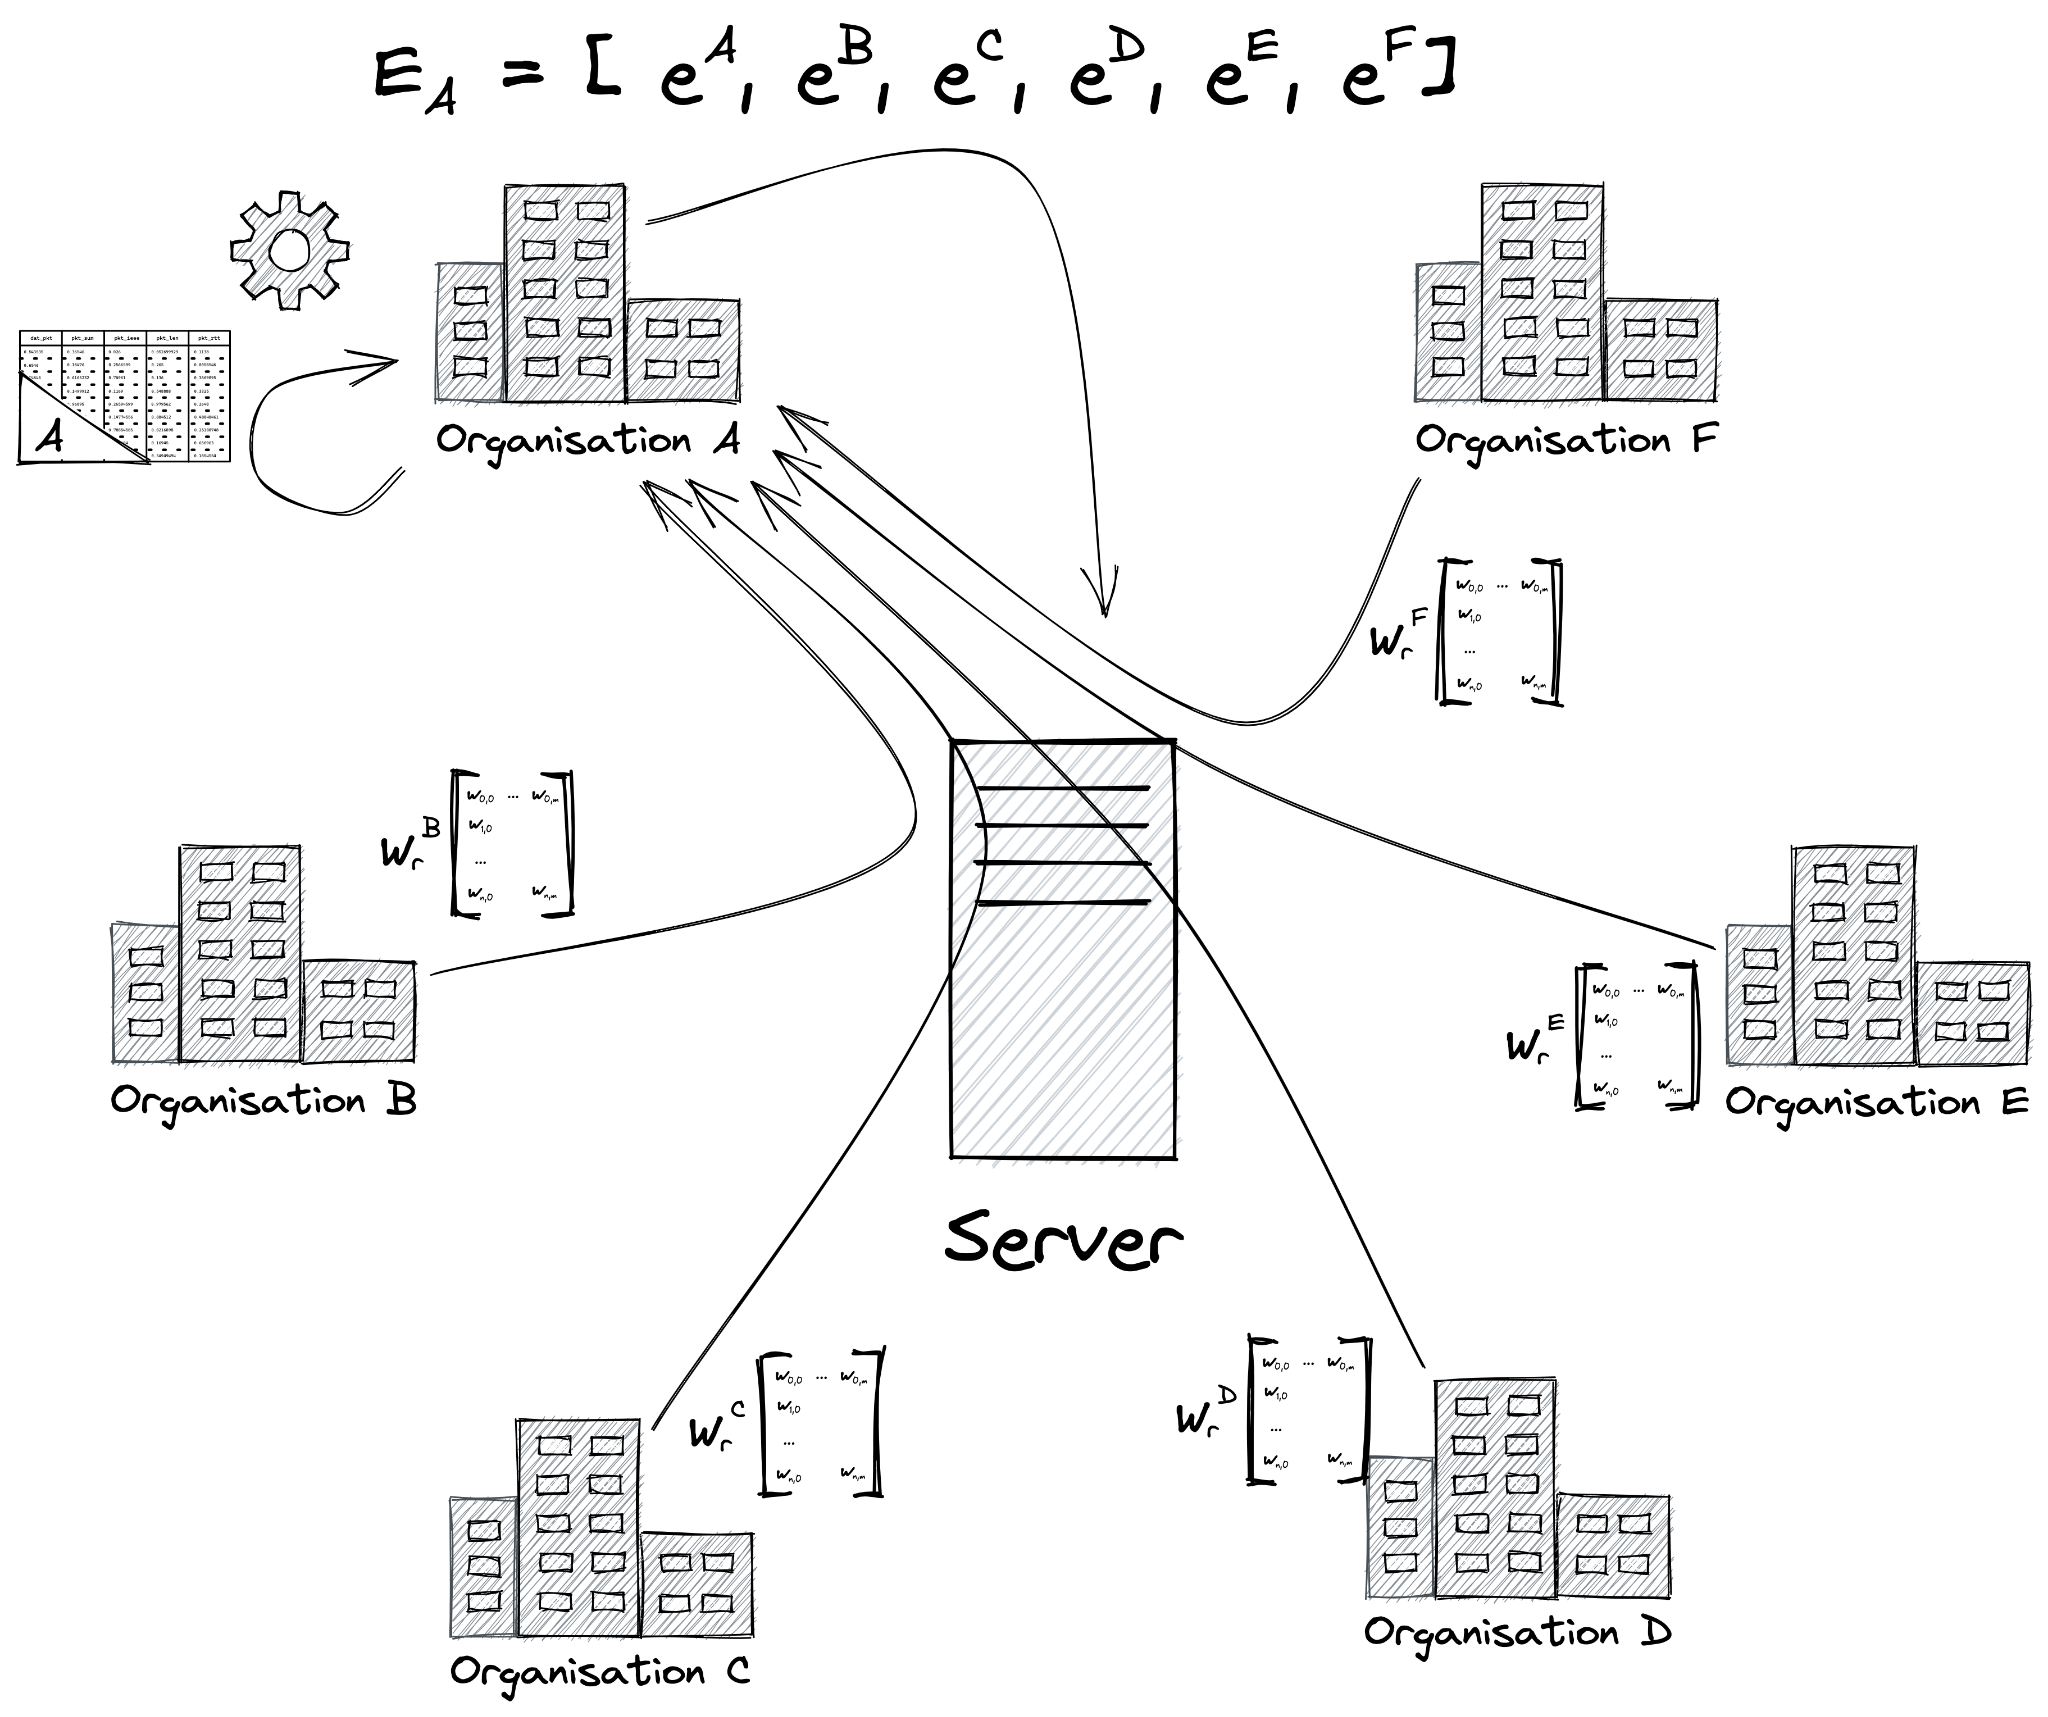
\includegraphics[width=\textwidth]{figures/radar/xeval}
      \end{figure}
    \end{column}
    
    \begin{column}{.55\textwidth}
      \small
      \setlength{\baselineskip}{0.8\baselineskip}
      \vspace{1ex}

      \textbf{Advantages}
      \begin{itemize}
        \item The central server does not need prior knowledge.
        \item Evaluates how each model fits the data (\eg, accuracy, F1 score).
        \item Exhaustive overview of the entire system at each round $r$.
      \end{itemize}

      \onslide<2->{%
        \textbf{Drawbacks}
        \begin{itemize}
          \item High communication and computation costs.
          \item Does not scale well.
          \item Shares local models to participants: less privacy-friendly.
        \end{itemize}
      }

      \onslide<3->{%
        \textbf{But\dots}
        \begin{itemize}
          \item Cross-silo use case: few clients, with reasonable computing capacity.
          \item Slow workflow: long time between rounds.
        \end{itemize}
      }   
    \end{column}

  \end{columns}

\end{frame}

\subsection{Fighting Heterogeneity with Clustering}
% Parler du thresold dynamique et de sa méthode de calcul. 
% 
\begin{frame}{Fighting Heterogeneity with Clustering}
  \begin{columns}
    \begin{column}{.55\textwidth}
      \textbf{Objective}
      \begin{itemize}
        \item Reduce heterogeneity for the aggregation.
        \item Build communities of \emph{more} homogeneous participants.
      \end{itemize}


      \onslide<2>{%
        \textbf{Clustering for FL}
        \begin{itemize}
          \item Regarding data-source:
          \begin{itemize}
            \item Gradient/model similarity.~\autocite{briggs_Federatedlearninghierarchical_2020}
            \item Cross-evaluation results.
          \end{itemize}

          \item Clustering methods:
          \begin{itemize}
            \item Dynamic \emph{split-and-merge}.~\autocite{chen_ZeroKnowledgeClustering_2021}
            \item Hierarchical clustering.~\autocite{briggs_Federatedlearninghierarchical_2020}
          \end{itemize}
        \end{itemize}
      }
      
    \end{column}
    \begin{column}{.45\textwidth}
      \begin{figure}
        \centering
        \makebox[\textwidth][c]{%
          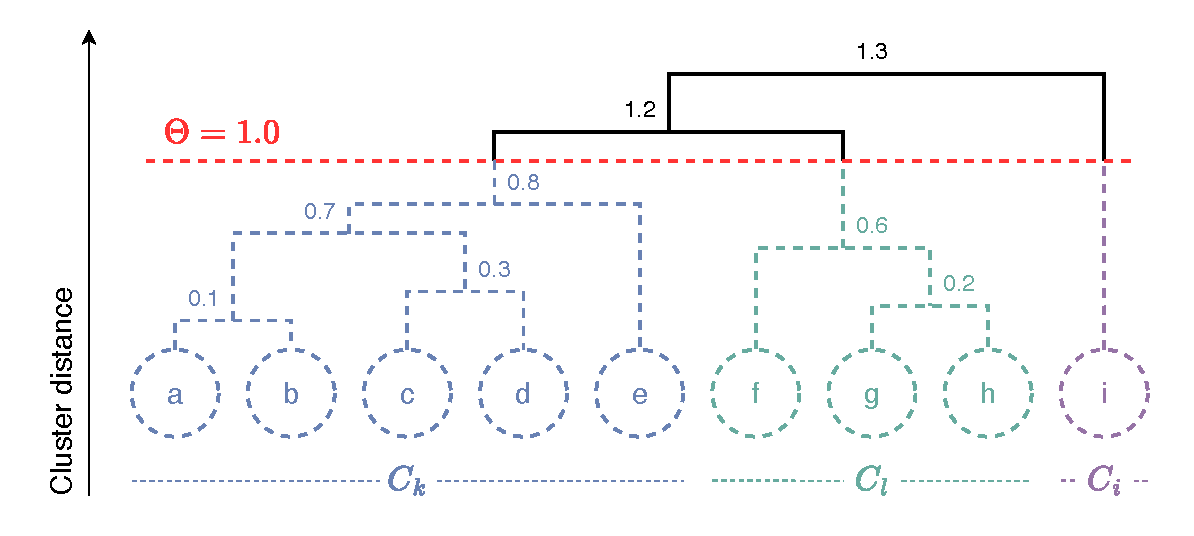
\includegraphics[width=1.2\textwidth]{figures/radar/clustering.drawio.pdf}%
        }
        %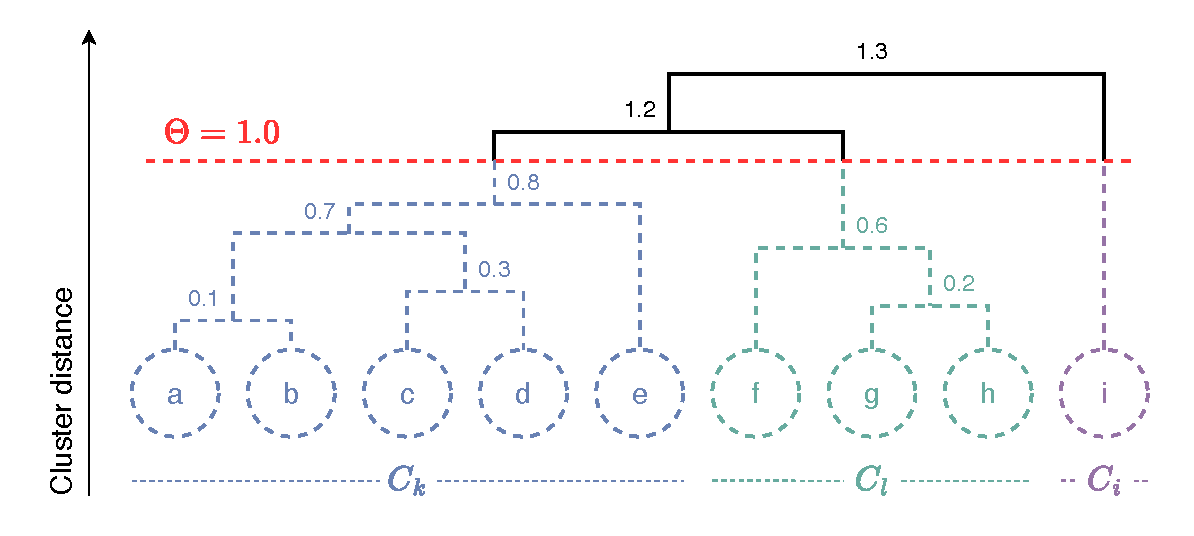
\includegraphics[width=\textwidth]{figures/radar/clustering.drawio.pdf}
        \caption{Hierarchical clustering.}
      \end{figure}
    \end{column}
  \end{columns}
  

  \only<2>{%
    \fcitefootnote{briggs_Federatedlearninghierarchical_2020}
    \fcitefootnote{chen_ZeroKnowledgeClustering_2021}
  }

\end{frame}

\subsection{Mitigating Byzantine Contributions}

\begin{frame}{Reputation-aware Aggregation}

  \begin{block}{Definition: Reputation Systems\normalfont~\autocite{resnick_Reputationsystems_2000}}
    \begin{itemize}
      \item Long-lived entities that inspire an expectation of future interaction;
      \item Capture and distribution of feedback about current interactions (such information must be visible in the future); and
      \item Use of feedback to guide trust decisions.
    \end{itemize}
  \end{block}

  \onslide<2>{%
    \begin{itemize}
      \item Dirichlet distribution for local aggregation of the reputation scores.~\autocite{fung_DirichletBasedTrustManagement_2011}
      \item Votes weighted by the similarity inside each cluster.
      \item Exponential decay for potential redemption.
    \end{itemize}
  }

  \fcitefootnote{resnick_Reputationsystems_2000}
  \only<2>{%
    \fcitefootnote{fung_DirichletBasedTrustManagement_2011}
  }

\end{frame}

